\documentclass[12pt, a4paper]{article}
\usepackage{scrextend}
\usepackage{titlesec}
\usepackage{graphicx}
\usepackage{amsmath}
\usepackage{amsfonts} % for the real number symbol
\usepackage{geometry}
\usepackage[unicode]{hyperref}
\usepackage{titlesec}
\usepackage{titletoc}
\usepackage[sorting=none]{biblatex}
\usepackage{xurl}
\usepackage{enumitem}
\usepackage{indentfirst}
\numberwithin{equation}{section} % number equations by section
\renewcommand{\figurename}{Att.}
\renewcommand{\contentsname}{Saturs}
\renewcommand{\labelenumi}{\arabic{enumi})} % lists with 1)
\setlist{nosep}
\parindent=1cm
\linespread{1.213} % equivalent to 1.5 in word, experimentally.
\addbibresource{refs.bib}

\geometry{
    a4paper,
    lmargin=30mm,
    rmargin=20mm,
    tmargin=20mm,
    bmargin=20mm
}


\titleformat{\section}
    {\normalfont\large\bfseries}{\thesection . }{0.2em}{\MakeUppercase}
\titleformat{\subsection}
    {\normalfont\large\bfseries}{\thesubsection . }{0.2em}{}
\titleformat{\subsubsection}
    {\normalfont\normalsize\bfseries\itshape}{\thesubsubsection . }{0.2em}{}
\titlespacing*{\subsubsection}{0pt}{6pt}{0pt}

\begin{document}
\begin{titlepage}
    \begin{center}
        \vspace*{3cm}
        
        LATVIJAS UNIVERSITĀTE

        DATORIKAS FAKULTĀTE

        \vspace*{4cm}

        \large\textbf{COVID-19 IEROBEŽOŠANAS PROJEKTU PĀRVALDĪBAS ASPEKTI}
        
        \vspace{2cm}
        \normalsize{REFERĀTS IT PROJEKTU PĀRVALDĪBĀ}
         
             
    \end{center}
    \vspace{3cm}
    \begin{addmargin}[18em]{0em}
    Autors: \textbf{Pēteris Račinskis}
    \end{addmargin}

    \begin{addmargin}[18em]{0em}
    \hspace{1cm} Stud. apl. Nr. pr20015
    \end{addmargin}

         
    \vfill
    \begin{center}
    RĪGA 2022
    \end{center}
 \end{titlepage}
\newpage
\tableofcontents
\thispagestyle{empty}
\newpage
\setcounter{page}{3}


\section{Ievads}

Pagājuši nedaudz vairāk kā trīs gadi, kopš parādījās pirmās ziņas, ka Uhaņā --- vienām no Ķīnas lielākajām pilsētām --- dažiem pacientiem konstatēta saslimšana ar iepriekš neredzētu infekcijas slimību. Tās simptomi atgādina gripu, taču vīruss nepieder pie gripas vīrusu dzimtes --- tas ir jauns, potenciāli ārkārtīgi lipīgs koronavīruss. Iepriekšējā reize, kad Ķīnā atklāts cilvēkam bīstams koronavīruss, bijusi 2002. gada rudenī, kad sākusies nāvējošā, taču mērogā samērā ierobežotā SARS epidēmija. Sociālajos tīklos šīs ziņas strauji sasniedz visu pasauli, medicīnas aprindās virmo satraukums, taču rietumos plašsaziņas līdzekļi un sabiedrība kopumā lielu uzmanību tām nepievērš --- jaunu, bīstamu vīrusu parādīšanās kaut kur tālu prom ir regulāra parādība, kas, par spīti dažādu pasaules gala solītāju vaimanāšanai, nekad taču pie nopietnām sekām šeit pie mums nenovedīs. 

Reti kurš toreiz, ap 2019/2020. gadu miju spēja iztēloties to, ka tikai dažus mēnešus vēlāk lielveikalu plauktus panikā tukšos ar tualetes papīru apkrāvušos cilvēku drūzmas un ziņas par miljonu nāvi būs vien fona troksnis, bet šobrīd --- 3 gadus vēlāk --- sadzīvošana ar epidemioloģiskajiem ierobežojumiem ir kļuvusi par ikdienu, vakcinācija --- par karstāko tematu politikā --- un grūti vairs atcerēties, kā dzīve norita pirms tam. Teikt, ka pēdējie daži gadi ir bijuši visnotaļ interesanti valdībām un nevalstiskajām institūcijām, kuru uzdevumis bijis novērst, ierobežot un pārvarēt pandēmijas sekas, būtu maigi. Krīzes vadības stratēģijas un plāni, kas desmitgadēm ilgi bijušas vien teorētiski domas lidojumi, izvilktas no atvilknēm un liktas lietā. Iepriekš neredzēti investīciju apjomi ieguldīti tradicionāli ļoti lēno medicīnas izstrādes un sertificēšanas procesu paātrināšanā. Nācies praktiski saskarties un dārgi maksāt par nevīžīgi veidotiem sabiedriskās domas procesiem. 

Kaut gan pandēmija vēl nebūt nav galā, pagājis pietiekami ilgs laiks, lai varētu pakāpties soli atpakaļ, atskatīties uz šo īpatnējo vēstures periodu un mēģināt izdarīt kādus spriedumus. Kas īsti tika darīts? Kāpēc? Vai izdevās?


\subsection{Referāta mērķis un struktūra}

Šī referāta mērķis ir identificēt un novērtēt nozīmīgākos COVID-19 pandēmijas izplatības ierobežošanas un seku apkarošanas ietvaros veiktos projektus, galvenokārt no suverēnu valstu valdību vai supranacionālu organizāciju skatapunkta. Tā kā šī krīze ir skārusi visu pasauli, ļoti daudzas un dažādas institūcijas ir bijušas iesaistītas šajā procesā. Pie tam faktiski nevienai nav iespējams visu periodu un visas veiktās darbības loģiski apvienot viena projekta ietvaros --- lai veiktu jebkādu analīzi nedrīkst ignorēt faktu, ka jebkuras institūcijas cīņa ar pandēmiju bijusi savstarpēji saistītu, bet atšķiramu projektu virkne. Nākamajā nodaļā tiek aprakstīts, pēc kāda principa nolemts izšķirt dažādus projektus, un kāpēc no ļoti daudzajiem sīkākai iztirzāšanai izvēlēti tieši tie, par kuriem runāts zemāk. Noslēgumā tiek apvienotas gūtās atziņas, izteikti subjektīvi novērtējumi un spriests par lietām, ko būtu bijis iespējams darīt labāk.

\newpage
\section{COVID-19 ierobežošanas projekti}

\subsection{Projektu dalījums un izvēle}

Lai būtu iespējams uz kādu darbību kopumu skatīties no projektu pārvaldības skatapunkta, nepieciešams vispirms saprast, kā tas iederas projekta jēdzienā. Atceroties semestra gaitā izstudētās ``\textit{Project Management Book}'' ievadā sniegto definīciju \cite{proj_book_intro} un nedaudz pārfrāzējot, projektu var definēt kā darbību ar sekojošajām īpašībām:

\begin{enumerate}
    \item tā ir vienreizēja un izpildāma noteiktā laikā --- ja kaut kas tiek darīts daudzkārt vai atkārtots nebeidzami, tas jau ir process. Procesa ieviešana ir projekts, bet ne pats process;
    \item tai ir skaidri definēts sākums un noslēgums;
    \item no tās tiek sagaidīts konkrēts rezultāts --- sasniegts mērķis;
    \item tai piešķirti konkrēti resursi;
    \item tās izpildi vada skaidri definēta projekta vadības hierarhija. 
\end{enumerate}

Tātad pilnīgi patvaļīgi izvēlēties kādu tematu un sākt tam piemērot projektu vadības terminoloģiju nav pareizi. Pandēmijas apkarošana ir ļoti garš un kopumā nestrukturēts process. Pat ja izvēlamies kādu konkrētu organizāciju --- piemēram, Latvijas Republikas Ministru kabinetu --- nav iespējams definēt vienotu mērķi, resursus, vadības hierarhiju vai noslēguma nosacījumus visam šim pasākumam kopumā. Tāpēc jāievieš smalkāks un precīzāks dalījums apakšuzdevumos, kuriem visas projekta īpašības var piemērot.

Viena no pirmajām un sabiedrības prātos vispamanāmākajām darbībām, ko pasaules valstu valdības realizējušas, ir vīrusa izplatības ātruma samazināšanas līdzekļu pieņem-šana. Tas ticis darīts jau pašā laika posma sākumā, kad par slimību vēl bijis zināms visnotaļ maz, pieejamas bijušas tikai ļoti trulas un invazīvas metodes, kuru efektivitāte --- tikai aptuveni aplēšama. Lai tās varētu izteikt kā projektus, nepieciešams katru ārkārtas ierobežojumu ieviešanas stadiju --- reakciju uz augošas saslimstības ``vilni'' --- izdalīt atsevišķi. Tas ne vienmēr ir vienkārši, jo pastāvējušas dažādas pakāpeniskas ierobežojumu pastiprināšanas sistēmas, turklāt katra perioda noslēguma parasti ne visi pieņemtie līdzekļi ir atcelti. Tomēr kopumā iespējams definēt vismaz aptuvenu mērķi, sākumu un noslēgumu, sagaidāmos un sasniegtos rezultātus kā arī atbildīgo vadības hierarhiju katram pandēmijas vilnim.

Otra tēma, kas interesanta tieši no projektu pārvaldības viedokļa, ir vakcīnas. Šeit gan saskaramies ar sarežģījumu --- pirmajā pandēmijas gadā noritēja faktiski tikai vakcīnu izstrādes un testēšanas procesi, bet pēc tam jau izstrādātās vakcīnas nācies izmantot nepieredzēta apjoma imunizācijas kampaņā. Šie ir ļoti atšķirīgi uzdevumi ar dažādiem mērķiem, līdzekļiem un sagaidāmiem rezultātiem. Vakcīnu izstrāde un paātrinātā apstiprināšana lietošanai, kas notikusi pamatā ASV, Ķīnā un Krievijā 2020. gadā ir interesants temats, ko pienācīgi aplūkot šāda vispārīga referāta ietvaros nav iespējams. Tāpēc apksatīti tikai vakcinācijas pasākumi ar jau izstrādātajām vakcīnām Latvijā. Vakcinācija atdalīta no vīrusa izplatības ātruma mazināšanas projektiem, jo vakcinācijai nosprausti mērķi ilgākos termiņos un tā noris paralēli vairākiem ierobežojumu ieviešanas etapiem.

\subsection{Vīrusa izplatības tūlītēja samazināšana}

Epidēmijas vēršas plašumā eksponenciāli. Ja zināms, ka vīruss ir pietiekami lipīgs, lai katru dažu dienu laikā dublutotu saslimušo skaitu, valdības jau vairākas nedēļas pirms krīzes sliktākā punkta ir nostādītas fakta priekšā --- ja nekas netiks darīts, inficēto skaits pārvarēs veselības aprūpes sistēmu spēju tos aprūpēt, un mirs daudzi, kas citādi būtu no tā izvairījušies. Īsie laika periodi spiež izmantot tos līdzekļus, kas tajā brīdī ir pieejami --- pat ja tie ir potenciāli postoši tautsaimniecībai un nepopulāri sabiedrībā. Tieši šis faktors var radīt sarežģījumus, jo demokrātiskās sistēmās valsts vadība ir atbildīga vēlētāju priekšā. Tādi var rasties interešu konflikta situācijas, kad ieviest optimālo risinājumu nav iespējams.

\subsubsection{Pirmie viļņi --- starptautisks salīdzinājums}

Lai gan pandēmijas sākums meklējams Ķīnā, 2019. gada nogalē, un tur arī tika realizēts pirmais nopietnais vīrusa apkarošanas projekts 2020. gada pirmajos mēnešos, ļoti maz kas ir zināms par šīs nedemokrātiskās valsts iekšējiem lēmumu pieņemšanas procesiem. Taču tieši tur tika iegūta pirmā informācija par infekcijas īpašībām, kas kalpoja par pamatu citur pieņemtajiem lēmumiem --- vīrusa izplatības veidi, aptuvenā mirstība, simptomi, ģenētiskais kods (kas ļāvis izstrādāt testus un vakcīnas). Grūti objektīvi novērtēt pirmo atbildi, jo to nav ar ko salīdzināt --- citām valdībām jau projekta definīcijas stadijā bijis pieejams ievērojami vairāk informācijas par problēmu. 

Tāpēc nolemts apskatīt un salīdzināt reakcijas sekundārās infekcijas valstīs, lai radītu priekštatu par faktoriem, kas noved pie veiksmīgas izplatības viļņa novēršanas pat sliktākajos --- informācijas trūkuma un vispārējas nesagatavotības --- apstākļos. Iztirzāt visas nav iespējams, tāpēc nolemts izvēlēties ilustratīvus piemērus dažādām pieejām un to rezultātiem, kā arī Latvijā darīto. Parasti kontrastainas pieejas var atrast starp ASV, Eiropas Savienības un tālo austrumu valstīm. Pirmajam vilnim par piemēriem ņemti Taivānas, ASV un Latvijas ieviestie pasākumi.

Taivānu jeb Ķīnas Republiku varētu savā ziņā uzskatīt par idealizētu piemēru pandē-mijas pirmā viļņa pārvarēšanai \cite{Taiwan_wave_1}. Tā ir neliela sala, kas atvieglo robežu kontroles pasākumus, bet tai pat laikā cieši ekonomiski saistīta ar konkurējošo komunistisko Ķīnas režīmu, kas to jau pašā sākumā pakļāva ievērojamam epidmioloģiskam riskam. No organizatoriskā viedokļa, Taivāna baudījusi zināmas priekšrocības --- pēc 2003. gada SARS epidēmijas tika izveidota īpaša valdības aģentūra, kuras mērķis ir sagatavoties un koordinēt visu valdības līmeņu reakciju uz epidemioloģiskiem draudiem --- \textit{National Health Command Center} (NHCC) \cite{wang2020response}. Šāda veida pastāvīga organizācija ievērojami atvieglo krīzes vadības uzdevumu --- nav nepieciešams veidot projekta hierarhiju un risināt resursu pārdales konfliktus, ja jau lacīgi sagatavoti reakcijas plāni, sadalīta atbildība par pienā-kumiem un rezervēti resursi risinājumu ieviešanai. Plašais un vispārīgais saslimstības viļņa ierobežošanas projekts tiek reducēts uz procesu, kura gaitā tiek sistemātiski ieviesti mazāki, kodolīgāki projekti konkrētu darbību veikšanai. 

Pirmās darbības tika veiktas jau pašā 2020. gada sākumā, kad ļoti maz kas bijis zināms par Ķīnā konstatēto jauno infekcijas slimību --- sāktas veselības pārbaudes ieceļotājiem no Ķīnas. Ārkārtas komandcentrs NHCC tika aktivizēts jau 2020. gada 20. janvārī, tajā pašā dienā, kad Ķīnas valdība pirmo reizi apstiprināja, ka infekciju iespējams pārnest no cilvēka uz cilvēku \cite{human_human}. Nākamā mēneša laikā komandcentra vadībā tika operatīvi realizēta virkne projektu ar mērķi nepieļaut vīrusa izplatību sabiedrībā --- jaunā mācību semestra sākuma pārbīde, ierobežojumi masu pasākumiem, pastiprināta robežkontrole un ceļošanas aizliegumi, karantīnas režīma ieviešana ceļotājiem, ekstensīva testēšana un kontaktu izsekošana. Turklāt ļoti operatīvi tika ieviestas izmaiņas veselības aprūpes IT sistēmās, lai būtu iespējams izsekot indivīdu ceļošanas vēsturei \cite{wang2020response}. Tā kā Taivāna kopā ar Ķīnu toreiz bijušas starp vadošajām medicīnisko masku ražotājām pasaulē, ieviests masku eksporta aizliegums ar mērķi saglabāt vietējās rezerves \cite{export_ban} --- kas gan, iespējams, ir viens no iemesliem neskaidrajai informācijai par sejas masku nepieciešamību, ko rietumvalstu valdību pārstāvji devuši sabiedrībai 2020. gada pavasarī ar mērķi novērst deficītu \cite{backfired}. Sākotnēji arī Taivānā sejas masku lietošana nav bijusi obligāta, taču pieaugot saslimstībai šis lēmums ticis mainīts \cite{taiwan_mask}. 

Kopumā var teikt, ka šie pasākumi vainagojās ar izciliem rezultātiem. Par spīti Taivānas ģeogrāfiskajai tuvībai un ciešajām ekonomiskajām saitēm ar pandēmijas sākum-punktu, līdz 2020. gada 30. jūnijam kopējais reģistrēto saslimšanas gadījumu skaits valstī bija 447, ar 7 nāves gadījumiem \cite{taiwan_stats} --- valstī ar 23,8 miljoniem iedzīvotāju \cite{taiwan_pop}. Tā gada pavasarī un vasarā bijuši ilgāki periodi bez jauniem inficēšanās gadījumiem \cite{taiwan_zero}. Pat ja reālie saslimstības rādītājie bijuši daudzkārt lielāki, šis rezultāts pirmā viļņa ietvaros bijis viens no labākajiem pasaulē. Un tas viss --- bez smagu mājsēdes pasākumu ieviešanas, jo lielākoties izdevies izvairīties no vīrusa izplatības sabiedrībā un apraut infekcijas ķēdes.

Savukārt ASV reputācija pirmā pandēmijas viļņa gaitā tika stipri iedragāta. 2020. gada pavasarī un vasarā absolūtā saslimšanas gadījumu skaita ziņā šī valsts dominēja. Turklāt, atšķirībā no daudzām citām pasaules valstīm, ar vasaras pienākšanu vīrusa izplatība nepierima --- tā vietā vasaras laikā varēja novērot vēl vienu saslimšanas gadījumu skaita pieaugumu \cite{us_stats}.

Noderīgi salīdzināt tieši aspektus, kas atšķirīgi starp ASV un Taivānu:

\begin{enumerate}
    \item Taivāna ir neliela, unitāra valsts. ASV ir ļoti liela, federāla valsts, kuras pavalstīm ir plašas pilnvaras, un liela daļa valsts institūciju resursu tiek kontrolēti tieši caur šo pavalstu līmeni. Loģiski, ka Taivānai un citām unitārām valstīm ir vieglāk ieviest vienotu pandēmijas apkarošanas politiku;
    \item starp ASV pavalstīm pastāv konstitucionāli garantētas tirdziniecības un pārvieto-šanās brīvības \cite{us_movement}. Pavalstis, kur ieviesti stingrāki ierobežojumi, nevar viegli apturēt kontaktu ar citām, kurās vīruss plosās neierobežoti. Tāpēc arī lokāli, pavalstu līmenī nav iespējams realizēt suverēnās valstīs populāro ieceļošanas aizliegumu politiku;
    \item epidemioloģiskie ierobežojumi ir jautājums, kas rada politiskas domstarpības. Masu pulcēšanās aizliegumi, skolu aizvēršana, uzņēmējdarbības u.c. ierobežojumi visi rada tūlītējus zaudējumus tautsaimniecībā, savukārt mirstības izraisītie nav tik viegli redzami, un to apjomu ir grūti novērtēt teorētiski. Daudzviet pasaulē politiskajā sfērā stipri pārstāvētas to sabiedrības daļu intereses, kas tieši izjūt ierobežojumu negatīvās ekonomiskās sekas --- varbūt nekur tik spēcīgi, ka ASV republikāņu partijā, kas tradicionāli kontrolē daudzus valsts centrālos štatus un 2020. gadā --- arī prezidenta adminstrāciju un parlamenta augšpalātu \cite{congress_2020}. Šķiet pašsaprotami, ka jebkura projekta realizācija tiek stipri apgrūtināta, ja tā vadība ir pakļauta interešu konfliktiem. Salīdzinājumam --- Taivānas viceprezidents kritiskajā pirmā viļņa periodā līdz 2020. gada maijam bija epidemioloģijas profesors \cite{taiwan_vp}, kas netieši liecina par faktu, ka vismaz toreizējā administrācijā medicīnas aprindu intereses epidemioloģiskajos jautājumos bijušas pārstāvētas.
\end{enumerate}

Šo faktoru kombinācija novedusi pie smagiem rezultātiem. Tieši ASV savulaik tikusi uzskatīta par vadošo pasaules valsti slimību apkarošanā --- \textit{Centers for Disease Control and Prevention} (CDC), ASV federālā sabiedrības veselības aģentūra, dibināta malārijas epidēmiju apkarošanai \cite{parascandola1996mcwa} un kalpojusi par piemēru līdzīgām institūcijām citur pasaulē. Starp tām ir gan Taivāna --- kuras NHCC aktivizēšana bijusi tās analoģiski nosauktās CDC uzdevums \cite{wang2020response} --- gan Latvija, par ko liecina slimību profilakses un kontroles centra (SPKC) nosaukums angļu valodā \cite{spkc_lv}. Taču par spīti atbildīgās valdības organizācijas pastāvēšanai, nav tikusi izveidota Taivānas NHCC ekvivalenta visaptveroša krīzes vadības sistēma un 2020. gadā ASV neizdevās efektīvi ierobežot vīrusa izplatību. Vispirms smagi skarti tikuši blīvāk apdzīvotie, urbanizētie štati, bet pēc tam vasarā vairāk cietušas valsts centrālās pavalstis \cite{us_stats}. Daudzviet notikusi pāragra ierobežojumu atcelšana, kas, iespējams, bijusi politisku apsvērumu motivēta \cite{florida_cancel}. Šī augstā saslimstības rādītāja dēļ 2020. gada vasarā ASV ir grūti pat skaidri nodalīt pirmo vilni no otrā --- pirmo reizi vīrusa izplatība manāmi ierobežota tikusi tikai 2021. gada vasarā, kad vakcinācija jau noritēja pilnā tempā un bija nomainījusies valsts administrācija.

Lietojot vienu un to pašu mērogu grafikā, uz vēlāko fona pirmais saslimstības vilnis Latvijā vispār nav redzams --- jūnija beigās kopējais konstatēto saslimšanas gadījumu skaits bijis 1118, bet nāves gadījumu --- 30 \cite{lv_stats}. 2020. gada sākumā, kad vīrusa starptautiskā izplatība vēl tikai nesen bija sākusies, Latvijas situācija bija diezgan padevīga veiksmīgai ierobežojumu ieviešanai. Tāpat kā Taivāna, Latvija ir neliela, unitāra valsts ar centralizētu veselības aprūpes sistēmu. Ģeogrāfiskais novietojums arī ievērojami samazinājis tiešo kontaktu ar epidēmijas skartajiem reģioniem Ķīnā, dodot atbildīgajām institūcijām vairāk laika pielāgoties situācijai kā arī piekļuvi citviet gūtām zināšanām un tehnoloģijām --- izplatības samazināšanas metodēm un COVID testiem. Kaut gan esam Eiropas Savienībā un Šengenas Līguma zonā, kā suverēna valsts paturam tiesības pārtraukt kustību pār savām robežām. Tobrīd sabiedriskajā domā izteikti viedokļi par vīrusa bīstamību un ierobežojumu vajadzību vēl nebija nostablizējušies, kas deva Ministru kabinetam politisku rīcības brīvību. Divu nedēļu periodā pēc pirmā Latvijā konstatētā saslimšanas gadījuma \cite{lv_first_case} tika izsludināts ārkārtas stāvoklis un sākās agresīva ierobežojumu ieviešana \cite{lv_measures}. 

Dažādo 2020. gada pavasara gaitā ieviesto noteikumu vidū bija tādas metodes kā skolu slēgšana un pāriešana attālinātā mācību režīmā, masu pasākumu liegumi, aizliegumi pulcēties vairāk nekā diviem cilvēkiem, ierobežojumi un papildus higiēnas prasības sabiedriskās ēdināšanas uzņēmumu darbā, divu metru distances prasības, sejas masku lietošanas prasības sabiedriskajā transportā u.c. Vēlāki pētījumi radījuši šaubas par dažādu pielietoto paņēmienu --- piemēram, skolu slēgšanas \cite{walsh2021school} --- efektivitāti, kas, kopā ar zemo saslimstību pirmā viļņa gaitā, droši vien palīdzējis sabiedrībā nostiprināties pret ierobežojumiem vērstiem viedokļiem. SPKC vadībā notikusi intensīva testēšanas un kontaktu izsekošanas programma, kurai izdevies apzināt lielu daļu no saslimšanas ķēdēm. Pienākot vasarai ārkārtas stāvoklis tika izbeigts un dažādie ierobežojumi --- pakāpeniski mīkstināti \cite{lv_reopen}, bet saslimstības rādītāji saglabājās zemā līmenī \cite{lv_stats}. 

Kopumā vērtējot Latvijas atbildi uz pirmo pandēmijas vilni, jāsecina, ka reaģēts tika ātri un agresīvi, taču nav skaidrs, cik efektīvi. Netika izveidota vienota atsevišķa projekta vadības sistēma tieši COVID-19 izplatības ierobežošanai, tā vietā tika izsludināts ārkārtas stāvoklis, kura ietvaros Ministru kabinets tiešā viedā uzņemas krīzes vadību \cite{lv_mk_control} --- pa vidu visiem citiem šīs organizācijas pienākumiem. Valdība diktējusi virkni ierobežojumu, taču grūti spriest, kuri no tiem patiešām ietekmējuši epidemioloģisko situāciju valstī. Latvijā nav iepriekš pastāvējis nekas pielīdzināms Taivānas NHCC, un nekas tāds arī nav ticis izveidots. Tā vietā viss pandēmijas apkarošanas process izteikts kā projekts ar neskaidri definētiem mērķiem un termiņiem, kura ietvaros notikusi \textit{ad hoc} lēmumu pieņemšana. 

\subsubsection{Vēlāki vilņi --- Latvijā}

Pēc sākotnējās atbildes uz jaunā koronavīrusa parādīšanos dažādu valstu stratēģiju salīdzinājumi kļūst mazāk informatīvi, jo ļoti liela nozīme ir iepriekšējiem notikumiem, kas ir atšķirīgi. Tā vietā sķiet interesantāk salīdzināt, kā vienas un tās pašas valsts problēmas risināšanas pieeja mainījusies laika gaitā. Pēc pirmā viļņa iespējams izšķirt trīs citus --- otro no 2020. gada oktobra līdz 2021. gada maijam vai jūnijam, trešo sākot no 2021. gada oktobra līdz 2021. gada decembra beigām, un ceturto --- 2022. gada sākumā, kad vīrusa populācijā notikušas izmaiņas un sācis dominēt $o$-variants \cite{lv_omicron_dominate}, piespiežot valdību reaģēt uz jaunu saslimstības paasinājumu pēc tam, kad jau izdevies to samazināt ar iepriekš izplatītajiem paveidiem.  

Ja reakciju uz pirmo vilni varētu raksturot kā pārlieku agresīvu, tad par otro drīzāk varētu sacīt, ka tā bijusi novēlota un negribīga. Atšķirībā no pavasara, kad ārkārtas stāvoklis tika izsludināts jau pēc pirmajiem dažiem inficēšanās gadījumiem, valdības reakcija uz saslimstības pieaugumu 2020. gada septembrī un oktobrī bija visai pasīva, jo ticis sekots iepriekš noteiktam 4\% pozitīvu testu īpatsvara rādītājam \cite{lv_october_2020_spread}. Tobrīd pandēmijas apkarošanas līdzekļu klāsts nebija sevišķi atšķirīgs no gada sākumā pieejamā, atšķirīga bija galvenokārt gatavība tos likt lietā. Ārkārtas stāvoklis tomēr tika izsludināts --- 2020. gada novembrī --- un palika spēkā līdz 2021. gada aprīlim \cite{lv_emergency_2020_fall}. Tāpat kā iepriekš, Ministru kabinets uzņēmies tiešu vadību pār visu procesu, bez detalizētas plānošanas tālākā nākotnē vai konkrētiem lēmumu pieņemšanas kritērijiem reaģējot uz situāciju, atjaunojot jau iepriekš piemērotus ierobežojumus un ieviešot jaunus --- piemēram, vispārīgu sejas masku lietošanas prasību iekštelpās, komandantstundu. Ja pavasarī infekcijas ķēžu apsekošana bijusi praktiska epidēmijas apkarošanas metode, tad šoreiz tas vairs nav bijis iespējams. Sākoties 2021. gadam, pirmoreiz kļuvušas pieejamas arī vakcīnas, taču to ieviešana gada pirmajā pusē gājusi lēni --- un detalizēti aprakstīta nodaļā par vakcinācijas projektu. Kopumā šai periodā izdevies salgabāt saslimstību stabilā, taču nu jau daudz augstākā līmenī --- līdz 2021. gada 30. jūnijam, kad saslimstība atkal sasniegusi sezonālos minimumus, kopā inficēto skaits bijis 137,429, bet bojā gājušo --- 2513.

Nākamais vilnis 2021. gada nogalē jau atgādināja iepriekšējo, tikai lielākā apjomā. Gada gaitā veiktā vakcinācijas kampaņa nebija sasniegusi īpaši augstu sabiedrības aptveri --- oktobrī aptuveni puse valsts iedzīvotāju bijuši vakcinēti \cite{lv_vaccine_half_2021_october}. Pieaugot saslimstībai septembrī un oktobra sākumā, Ministru kabinets atkal izsludinājis ārkārtas stāvokli --- šoreiz jau uzreiz uz trīs mēnešiem --- un uzņēmies tiešu vadību pār situāciju \cite{lv_emergency_2021}. Oktobra otrajā pusē tika ieviests, iespējams, stingrākais ierobežojumu režīms --- mājsēde ar komandantstundu, skolu daļēju aizvēršanu un virkni ierobežojumu komercdarbībā \cite{lv_lockdown_2021}. Papildus arī pastiprināti vakcinācijas motivēšanas līdzekļi \cite{lv_fire_unvaccinated}. Rezultātā saslimstības rādītāji sākuši kristies jau novembra sākumā, un stabilizējušies zemākā līmenī decembra vidū --- kaut gan šis zemākais līmenis sakritis ar iepriekšējā gadā augstākajiem \cite{lv_stats}. Var secināt, ka šoreiz reakcija uz situāciju tomēr bijusi ātrāka, un krīze oktobrī tikusi pārvarēta ar līdzekļiem, kuru rezultāti tūlīt bijuši redzami --- tātad par spīti pastāvīgas šāda tipa projektu vadības struktūras trūkumam un ne visai veiksmīgajai vakcinācijas ieviešanai, Ministru kabinets institucionālā līmenī ir mācījies no iepriekšējām kļūdām, vismaz tieši saslimstības viļņu "gludināšanā" ar ierobežojumu ieviešanu. Kā piemēru tam var minēt šoreiz jau diezgan precīzi izvēlēto ārkārtas pilnvaru perioda garumu --- tas izsludināts uz trim mēnešiem, un trīs mēnešu laikā situāciju tik tiešām izdevies stabilizēt, vismaz līdz vīrusa populācijas nomaiņas brīdim. 

Jaunākais vilnis --- $o$ varianta izraisītais straujais pieagums 2022. gada sākumā --- šobrīd vēl noris pilnā sparā, tāpēc izdarīt kādus spriedumus par to būtu pāragri. Ņemot vērā jaunāko informāciju --- piemēram, augstos saslimstības rādītājus skolēnu vidū \cite{lv_sick_student} --- gan izskatās, ka daļa ierobežojumu, iespējams, tikuši atcelti pārāk ātri, jo par $o$-varianta sagaidāmo uzliesmojumu jau sen bijis zināms.

Atskatoties uz valdības veikto pēdējo divu gadu laikā, redzams, ka nekādi sistemātiski risinājumi šobrīd jau sezonālo COVID-19 saslimšanas viļņu bīstamības mazi-nāšanai vēl joprojām nav ieviesti. Sasniedzot neskaidri definētus un, iespējams, mainīgus saslimstības kritērijus, Ministru kabinets izsludina ārkārtas stāvokli uz neskaidru laika periodu, uzņemas tiešu vadību pār krīzes vadības procesu un sāk realizēt kādus pandēmijas apkarošanas pasākumus, pagarinot ārkārtas pilnvaru periodu pēc vajadzības. Pirmajā reizē epidēmiju gandrīz pilnībā izvedies novērst, bet reakcija, iespējams, bijusi pārāk agresīva. Otrajā reizē, varbūt cenšoties reaģēt mazāk stingri, pieļauti daudz augstāki saslimstības rādītāji un ārkārtas situācija pamatīgi ieilgusi. Trešajā reizē, par spīti augstā-kiem skaitliskajiem rādītajiem, šķiet, reakcija beidzot bijusi visai trāpīga --- taču tās sasniegto gandrīz tūlīt izdzēsis nākamais vīrusa variants, kas liecina, ka šādas vadības struktūras spēja pielāgoties jaunām situācijām ir ierobežota.

\subsection{Vakcinācija}

Paralēli sezonālo saslimšanas viļņu apkarošanai ar visiem attiecīgajā laika posmā pieejamajiem līdzekļiem, 2021. gada sākumā uzsākts sabiedrības masveida imunizācijas projekts ar jaunizstrādātajām vakcīnām pret COVID-19, kura mērķis ir kopumā mazināt nākamo viļņu bīstamību. Šis pasākums izrādījies nebūt ne triviāls, jo gandrīz visur pasaulē nācies saskarties ar ne tikai neizlēmību un atturību no sabiedrības puses, bet pat klaju opozīciju vakcinācijai. Šajā apakšnodaļā runāts tikai par vakcināciju Latvijā, jo tā iespējams apskatīt vienu konkrētu projektu. Turklāt darba autoram personīgi bijis pieejams daudz informācijas no primāriem avotiem --- mediķiem ģimenē.

\subsubsection{Pirmreizējā}

Vakcinācijas projekts Latvijā jau pašā sākumā izrādījies strīdīgs --- tūlīt pēc pirmo vakcīnas devu izsniegšanas, 2021. gada sākumā premjerministrs pieprasījis un panācis veselības ministres demisiju, pamatojot to ar vakcinācijas plāna nepietiekamību \cite{lv_minister_fired}. Šķiet, galvenie iemesli šai samērā radikālajai rīcībai bijuši pietiekami detalizēta projekta plāna neesamība un zemākā vadības līmenī patvaļīgi pieņemts lēmums atteikties no papildus vakcīnu devām situācijā, kad vēl nebija nodrošināts pietiekmi lielas to rezerves. Pēc veselības ministra nomaiņas, izstrādāts konkrētāks vakcinācijas plāns \cite{lv_vaxx_plan} --- kas, atšķirībā no nestrukturētās valdības rīcības, apkarojot kārtējo saslimšanas vilni, paredzēts ilgākam laikam, kaut gan jau tā publicēšanas laikā tas tomēr uztverts ar skepsi. 

Piemēram, lielu daļu devu bijis paredzēts izsniegt caur eksistējošo ģimenes ārstu prakšu sistēmu, turklāt sākumā vakcīnēšana tika organizēta pa vecuma kategorijām. Šī plāna daļa izrādījusies izteikti nereālistiska. \textit{mRNA} tipa vakcīnas nepieciešams uzglabāt ļoti zemās temperatūrās, jo ribonukleīnskābes ir ļoti nestabilas un ātri degradējas, temperatūrām paceļoties virs aptuveni $-70^\circ$C \textit{Pfizer} un $-20^\circ$C \textit{Moderna} izstrādātajām. Nav praktiski iespējams ne pārvietot, ne uzglabāt šādus medikamentus lielākajā daļā ģimenes ārstu prakšu, tāpēc piegādes uz tām tiek realizētas pa iepakojumam --- katrā parasti ir 10 devu, kas visas ir jāizlieto dažu dienu laikā. Lai veiktu piegādi, ģimenes ārstam nepieciešams savākt konkrētu skaitu cilvēku un tos visus vienā īsā laika posmā arī vakcinēt. Uzreiz redzams, ka papildus vēl šķirojot pacientus vecuma un citu riska grupu kategorijās, kopējais vakcinācijas aptveres process tiek stipri palēnināts --- daudzi, kas būtu spējīgi ierasties un saņemt devu ir spiesti gaidīt uz mazāku skaitu personu, ko nav tik vienkārši vienlaikus pierunāt ierasties uz vakcināciju. Šīs vakcīnu uzglabāšanas īpatnības nozīmē, ka daudz ātrāk būtu iespējams procesu pabeigt, to veicot centralizēti un vienlaikus apkalpojot maksimāli lielu cilvēku skaitu. Ieteikumus veidot vakcinācijas centrus no ģimenes ārstu puses šī referāta autors dzirdējis jau tūlīt pēc jaunā vakcinācijas plāna uzzināšanas. Protams, šis skatījums nav bijis vienbalsīgs --- 2021. gada sākumā daudzviet lielāks kavējošais faktors bijis tieši vakcīnu sagāde, kas mudinājis daļu ģimenes ārstu kritizēt centralizētu vakcinācijas centru ieviešanu \cite{vaxx_center_oppose}.

Lai vai kā, plāns ticis pieņemts. Vakcinācijas projekta pārvaldībai ātri tika izveidota atsevišķa, tieši šim mērķim paredzēta veselības ministrijas struktūrvienība --- vakcinācijas birojs \cite{vaxx_bureau_proposed} --- kuras komanda tika noformēta dažu nedēļu laikā \cite{vaxx_bureau_leadership}. Biroja nepieciešamība gandrīz tūlīt tika apstrīdēta un tika vākti paraksti tā likvidēšanai, tomēr beigās tas tika reorganizēts un saglabāts \cite{vaxx_bureau_reorganized}.


\subsubsection{Balstvakcinācija}


\newpage
\section{Secinājumi}

Literatūras analīzē sniegts īss un nebūt ne pilnīgs --- vai vienlīdzīgi sadalīts --- līdz šim par atdarinošo mašīnmācīšanos veiktās pētnieciskās darbības pārskats. Jau izvēloties, par kurām tēmām rakstīts plašāk, par kurām --- mazāk detalizēti --- iespaidu uz darba saturu ir atstājusi motivējošās problēmas specifika. Tagad nepieciešams pie tās atgriezties un novērtēt, kas no visa nozarē pētītā un izgudrotā attiecas uz darba ievadā aprakstīto uzdevumu --- mešanas kustību iestrādāšanu atkritumu vai citu objektu pārvietošanā.

\subsection{Svarīgākās atziņas}

\begin{figure}[t!]
    \centering
    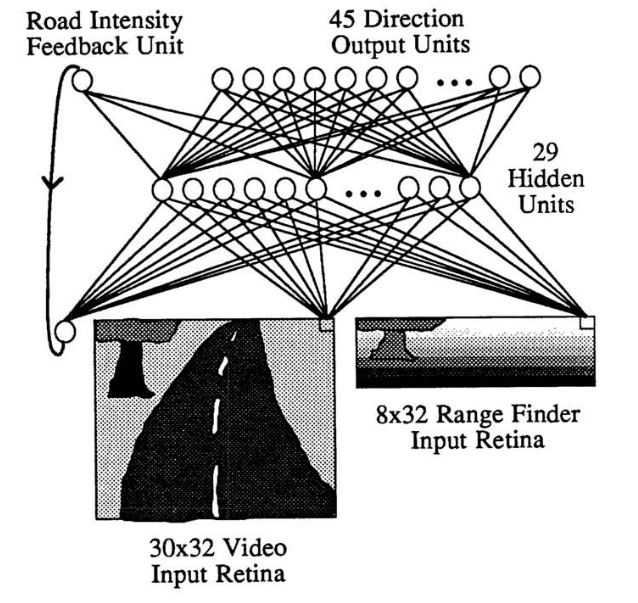
\includegraphics[height=6.8cm,page=1]{../img/alvinn_architecture.png}
    \caption{ALVINN modeļa uzbūve}
\end{figure}

\newpage
\addcontentsline{toc}{section}{Atsauces}
\printbibliography[title=Atsauces]

\end{document}